\documentclass[10pt,xcolor=pdflatex]{beamer}
\usepackage{newcent}
\usepackage[utf8]{inputenc}
%\usepackage[czech]{babel}
\usepackage{hyperref}
\usepackage{fancyvrb}
\usetheme{FIT}

%%%%%%%%%%%%%%%%%%%%%%%%%%%%%%%%%%%%%%%%%%%%%%%%%%%%%%%%%%%%%%%%%%
\title[FYO projekt]{Aberácie šošoviek}

\author[]{Roman Dobiáš}

\institute[]{Brno University of Technology, Faculty of Information Technology\\
Bo\v{z}et\v{e}chova 1/2. 612 66 Brno - Kr\'alovo Pole\\
xdobia11@stud.fit.vutbr.cz}

\date{May 15, 2019}
%\date{\today}
%\date{} % bez data

%%%%%%%%%%%%%%%%%%%%%%%%%%%%%%%%%%%%%%%%%%%%%%%%%%%%%%%%%%%%%%%%%%

\begin{document}

\frame[plain]{\titlepage}

\begin{frame}\frametitle{Aberácie šošoviek}
    \begin{itemize}
        \item čo to znamená ?
        \item ako vznikajú ?
        \item dôsledok ?
    \end{itemize}
\end{frame}

\begin{frame}\frametitle{Paraxialná optika}
    \begin{itemize}
        \item zjednodušenie pre \textbf{malé uhly} voči \textit{optickej osi}
    	\item sin x $\sim$ x

    	\item Snellov zákon - TODO

    	\item Obrázok geometrickej šošovky
        \begin{figure}
            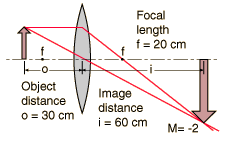
\includegraphics[scale=0.5]{img/thinLensEq.png}
            \caption{Model}
        \end{figure}
    \end{itemize}
\end{frame}

\begin{frame}\frametitle{Realita}
    \begin{itemize}
    	\item Upravený Schnellov zákon
    	\item Upravený Schnellov zákon pre chromatické vlny
    \end{itemize}
\end{frame}

\begin{frame}\frametitle{Rozdelenie aberácii}
    \begin{itemize}
        \item odchýlenie ľúčov od ohniskového bodu - Wikipedia
        \item \textbf{achromatické} \\
            \begin{itemize}
                \item rozostrenie
                \item deformácia 
            \end{itemize}
        \item \textbf{chromatické}
    \end{itemize}
    
\end{frame}


\begin{frame}\frametitle{Sférická aberácia}
    \begin{itemize}
        \item posunutie ohniska v závislosti na vzdialenosti od \textit{optickej osi}
        \item \textbf{Dôsledok:} rozostretý obraz 
        \item \textit{circle of the least confusion}
    \end{itemize}

    \begin{columns}
    \column{0.5\textwidth}
    \begin{figure}
        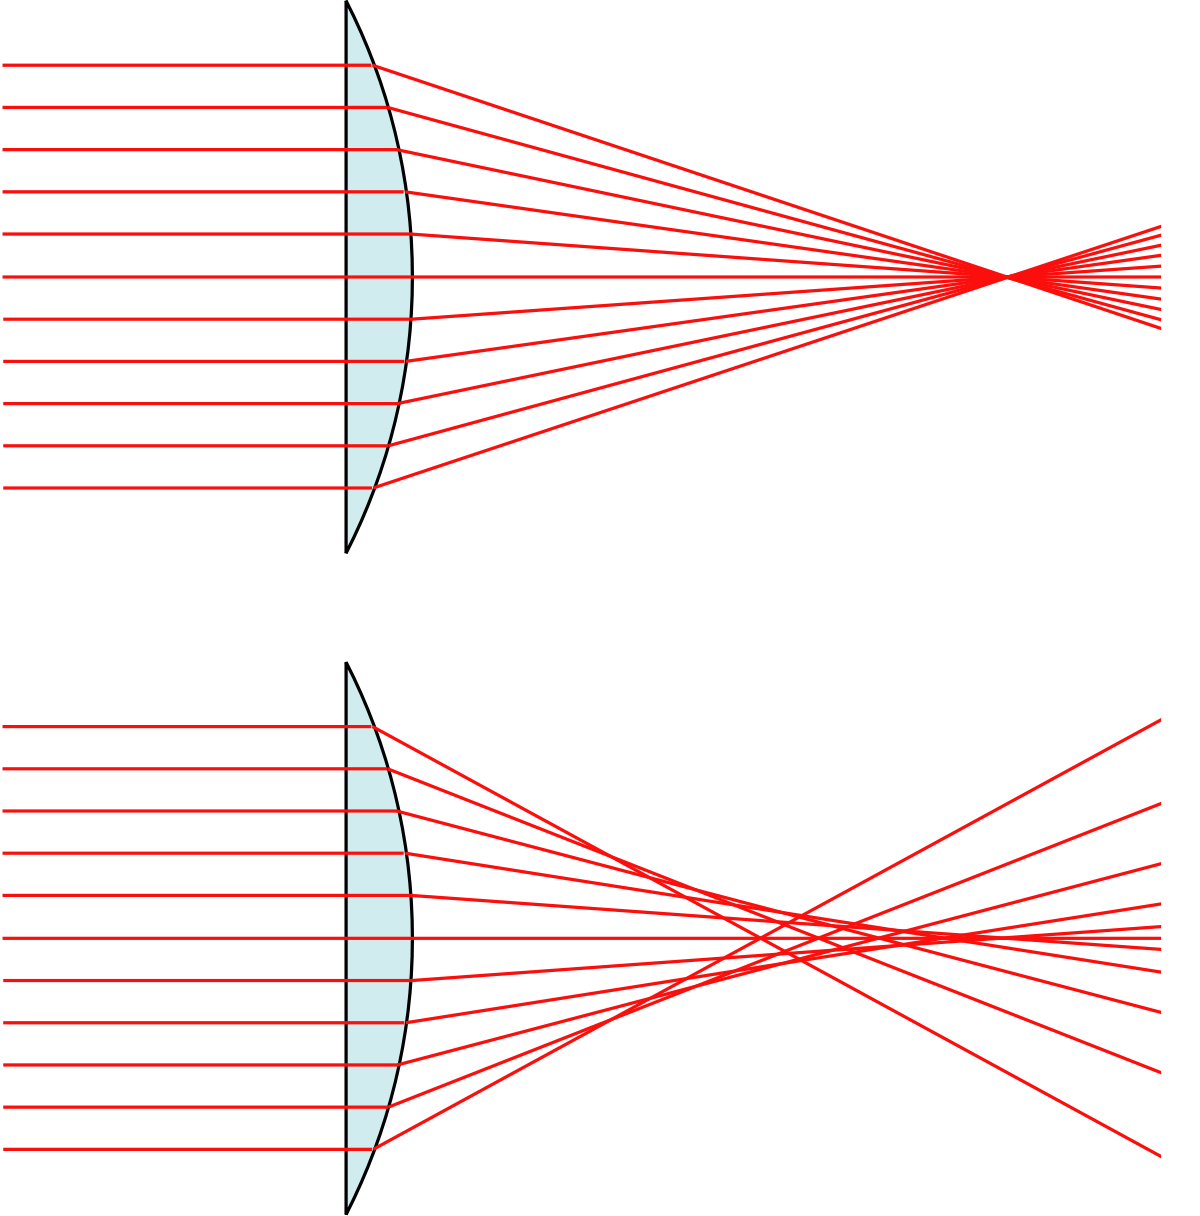
\includegraphics[scale=0.1]{img/sphericalAberrationWikipedia.png}
        \caption{Dôsledok aberácie => rozptyl ohnisk}
    \end{figure}
    \column{0.5\textwidth}
    \begin{figure}
        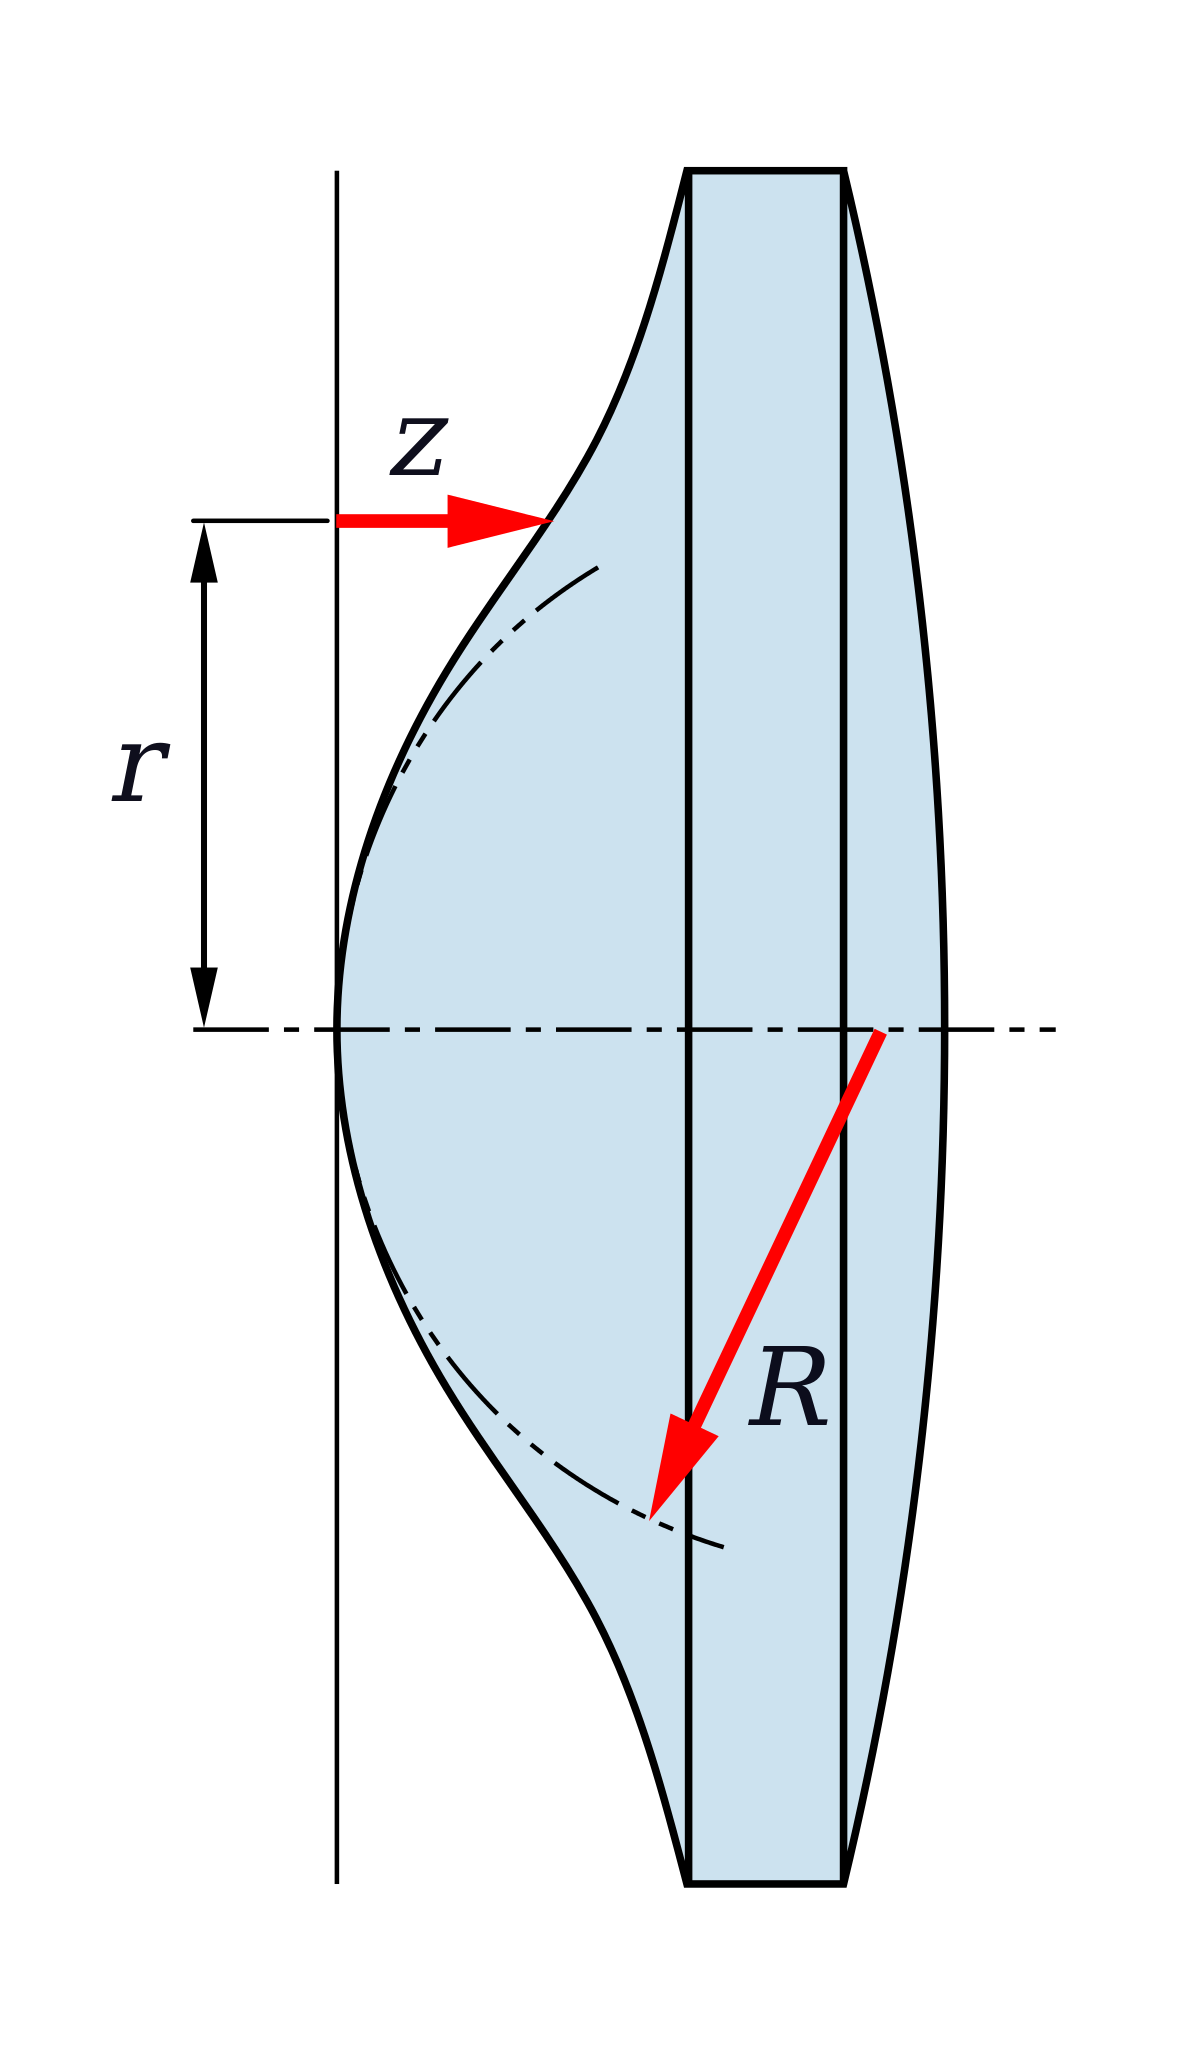
\includegraphics[scale=0.05]{img/asphericLen.png}
        \caption{Asférická šošovka}
    \end{figure}
    \end{columns}
        Riešienie: \textit{asférický tvar šošoviek}, korektory
\end{frame}

\begin{frame}\frametitle{Chromaticka aberácia}
    \begin{itemize}
        \item index lomu je funkciou \textbf{vlnovej dĺžky}
        \item \textbf{Dôsledok:} rozostrenie podľa farieb 
    \end{itemize}

    \begin{figure}
        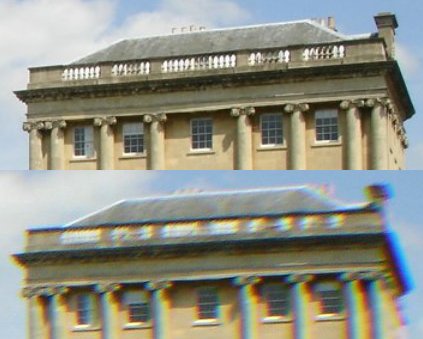
\includegraphics[scale=0.4]{img/chromaticAberrationWikipedia.jpg}
        \caption{lion!!}
    \end{figure}
    Riešienie: \textit{doublet}, SW korekcia 
\end{frame}

\begin{frame}\frametitle{Sférická aberácia}
    \begin{itemize}
        \item TODO
    \end{itemize}
\end{frame}

\bluepage{Ďakujem za vašu pozornosť / otázky}

\end{document}
